\section{Science Validation Survey}  \label{sec:svs}

\subsection{Operations Readiness Requirement}

The Project team shall conduct at least one autonomously driven Science Validation Survey with the science camera (LSSTCam) over a limited area of the sky that will last at least 30 days;

\subsection{Objectives}

The main objective of this criterion is to demonstrate the reliability of the as-built Rubin Observatory, meaning that hardware, software, and infrastructure functionality do not limit Observatory operations until the next programmed maintenance event.
To demonstrate reliability, one or more Science Validation Surveys will be conducted at the conclusion of the on-sky commissioning as a full rehearsal of science operations. The minimum 30-day time span for verification corresponds to $\sim 1\%$ of the 10-year LSST, and is intended to incorporate operations procedures over a full lunar cycle including:

\begin{itemize}
\item Filter swapping between bright and dark time;
%\item Management of survey scheduling during the period around full moon;
\item Active optics system, dome, and Scheduler response to a range of environment conditions encountered at the observatory over a 30-day period, including periods of cloud cover and variable atmospheric seeing, variable winds, and changes in daytime / nighttime temperature;
\item Response of the Data Management system to sustained data rates including simultaneous execution of the Alert Production and Data Release Production pipelines.
\end{itemize}

In addition, as a baseline, the following concepts of operations and their procedures will be rehearsed and demonstrated:

\begin{itemize}
\item Full rehearsal of safety procedures for science operations;
\item Scheduling shifts for daytime and nighttime operations;
\item Communication protocols for observation planning, daytime and nighttime operations and decision-making, and requesting support;
\item Routine daytime maintenance of the Observatory;
\item Collection and processing of routine calibration data and data products consistent with the time allotted in the 24-hour operations cycle;
\item Routine nighttime survey observing operations driven by the scheduler with minimal human interaction, including response to realtime telemetry, AuxTel;
\item Recovery from interruptions to observing (e.g., failure of the network)
\item Demonstration of near real time data quality assessment;
\item Prompt processing of alerts within the required latency time (i.e., 60 seconds);
\item Capability for distribution of Prompt products;
\item Prompt processing ``24-hour" data products (e.g., Solar System Object orbit calculations);
\item Cumulative Data Release Production with the full set of deep coadd and time-domain data products (at least once);
\item Access to on-sky data products via the Rubin Science Platform.
\end{itemize}

Data acquired during the Science Validation Survey(s) should routinely deliver acceptable science quality imaging to allow a summative assessment of the delivered scientific performance of the as-built system.
The Operations team plans to serve data products from the Science Validation Survey(s) as part of the Early Science Program \citeds{RTN-011}.

%\subsubsection{Baseline Sciece Validation Survey Design}


\textbf{Baseline Science Validation Survey Design}

(Updated June 2025)

On-sky engineering with LSSTCam began on 15 April 2025 and SV survey observations are expected to begin in late June 2025.
As more information regarding the progress of on-sky commissioning and plans for LSST Operations becomes available, Rubin Observatory has identified opportunities to refine the detailed implementation of the SV surveys to facilitate a smooth transition from Construction to Operations, and to enhance the potential impact of the Early Science Program.
The ``enhanced'' baseline SV survey design incorporates information regarding
\begin{itemize}
        \item the expected months of SV survey observations and visibility of specific target fields,
        \item overall operational efficiency and system performance demonstrated during the first two months of the on-sky commissioning campaign with LSSTCam,
        \item guidance derived from the community process to develop the LSST Cadence, facilitated by the Survey Cadence Optimization Committee (SCOC),
        \item input from the Rubin science community regarding the evolving scientific landscape and emergent opportunities,
        \item and planned engineering activities around the transition from Construction to Operations.
\end{itemize}

Rubin Observatory has developed and simulated a Feature Based Scheduler (FBS) configuration for the enhanced baseline SV survey design that could be implemented and is expected to meet the Construction completeness criteria if executed.

As of early June 2025, the forecast of on-sky commissioning activities includes pilot observations for the SV surveys beginning in late June, and sustained SV survey observations running from early July to mid September. The objectives of the SV survey pilot observations are to
\begin{itemize}
        \item evaluate the distribution of delivered image quality, including AOS performance, for wide-area survey observations,
        \item continue optimization of the AOS open loop and closed loop control systems,
        \item evaluate the overall operational uptime in wide-area survey mode observations similar to the nominal LSST cadence,
        \item and validate the FBS performance and the observing strategy for the SV surveys.
\end{itemize}

The enhanced baseline SV survey design includes two main survey components that are interleaved as part of a single FBS configuration:
\begin{itemize}
        \item a \textbf{Deep Survey} that is optimized for testing deep coadds at the equivalent integrated exposure of the LSST 10-year survey and beyond, achieving a rapid temporal sampling in those fields, and validating the observing strategy for the LSST Deep Drilling Fields (DDFs);
        \item a \textbf{Wide Survey} that is optimized for testing template generation and Prompt Processing with difference image analysis at data rates that would be expected during the first year of LSST, thereby providing a sustained full-scale test of the Data Facility;
\end{itemize}
The enhanced baseline SV survey adopts many of the design elements of the standard LSST cadence, with modifications to increase the likelihood of delivering a stand-alone high-impact dataset to enhance opportunities for Early Science.

For the SV surveys, a visit consists of a single 30 second exposure for $grizy$ and a single 38 second exposure for $u$.
The SV survey simulation assumes 55\% of time between evening and morning nautical twilight will be available for observations starting around 1 July 2025, with losses coming from weather, engineering downtime, and operation constraints.
The simulations assume that on-sky observations conclude 2 hours prior to sunrise, and a limited azimuth range 3 hours prior to sunrise.


\begin{figure}[htbp]
    \begin{center}
    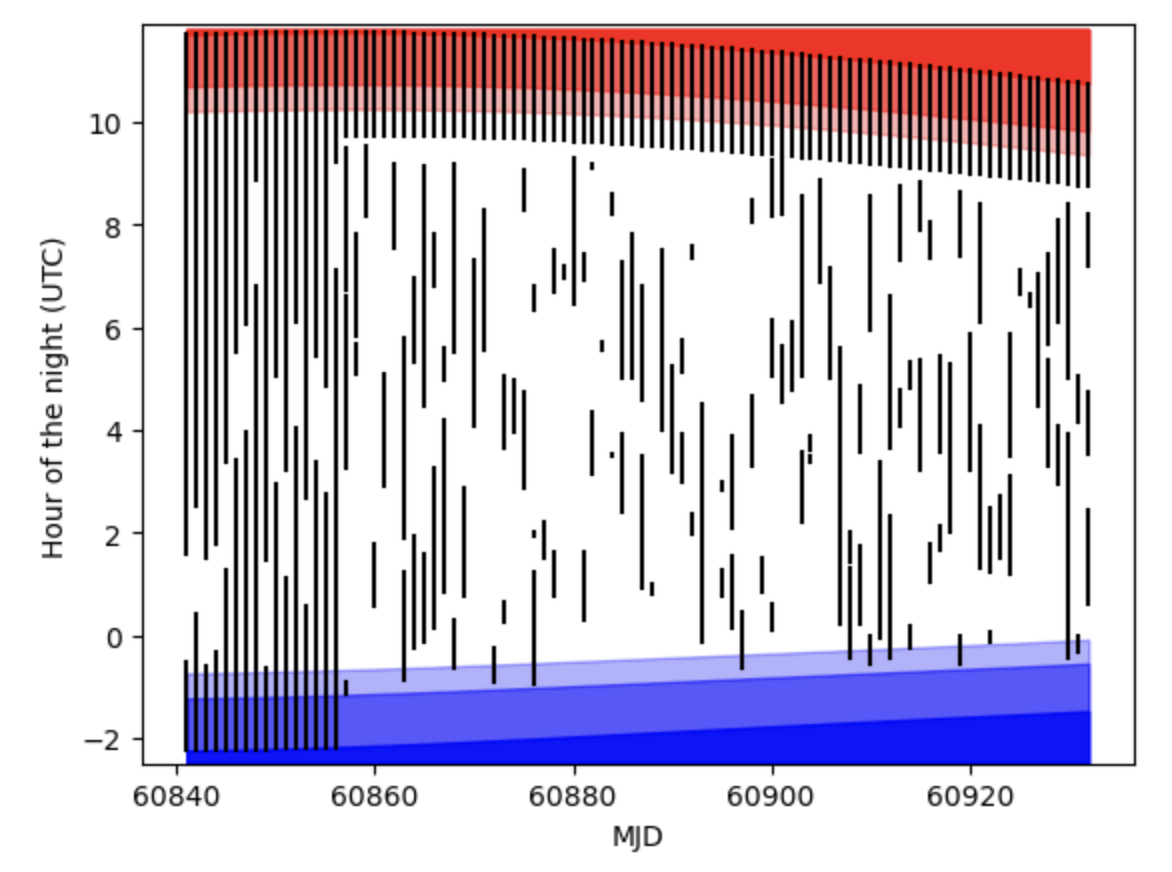
\includegraphics[width=1\textwidth]{./sv_surveys_uptime.png}
    \caption{SV surveys model of efficiency and engineering downtime used for the simulation. Black lines indicate engineering time. Shaded bands indicate evening and morning astronomical, nautical, and civil twilight periods.}
    \label{sv_surveys_uptime}
    \end{center}
\end{figure}

\begin{figure}[htbp]
    \begin{center}
    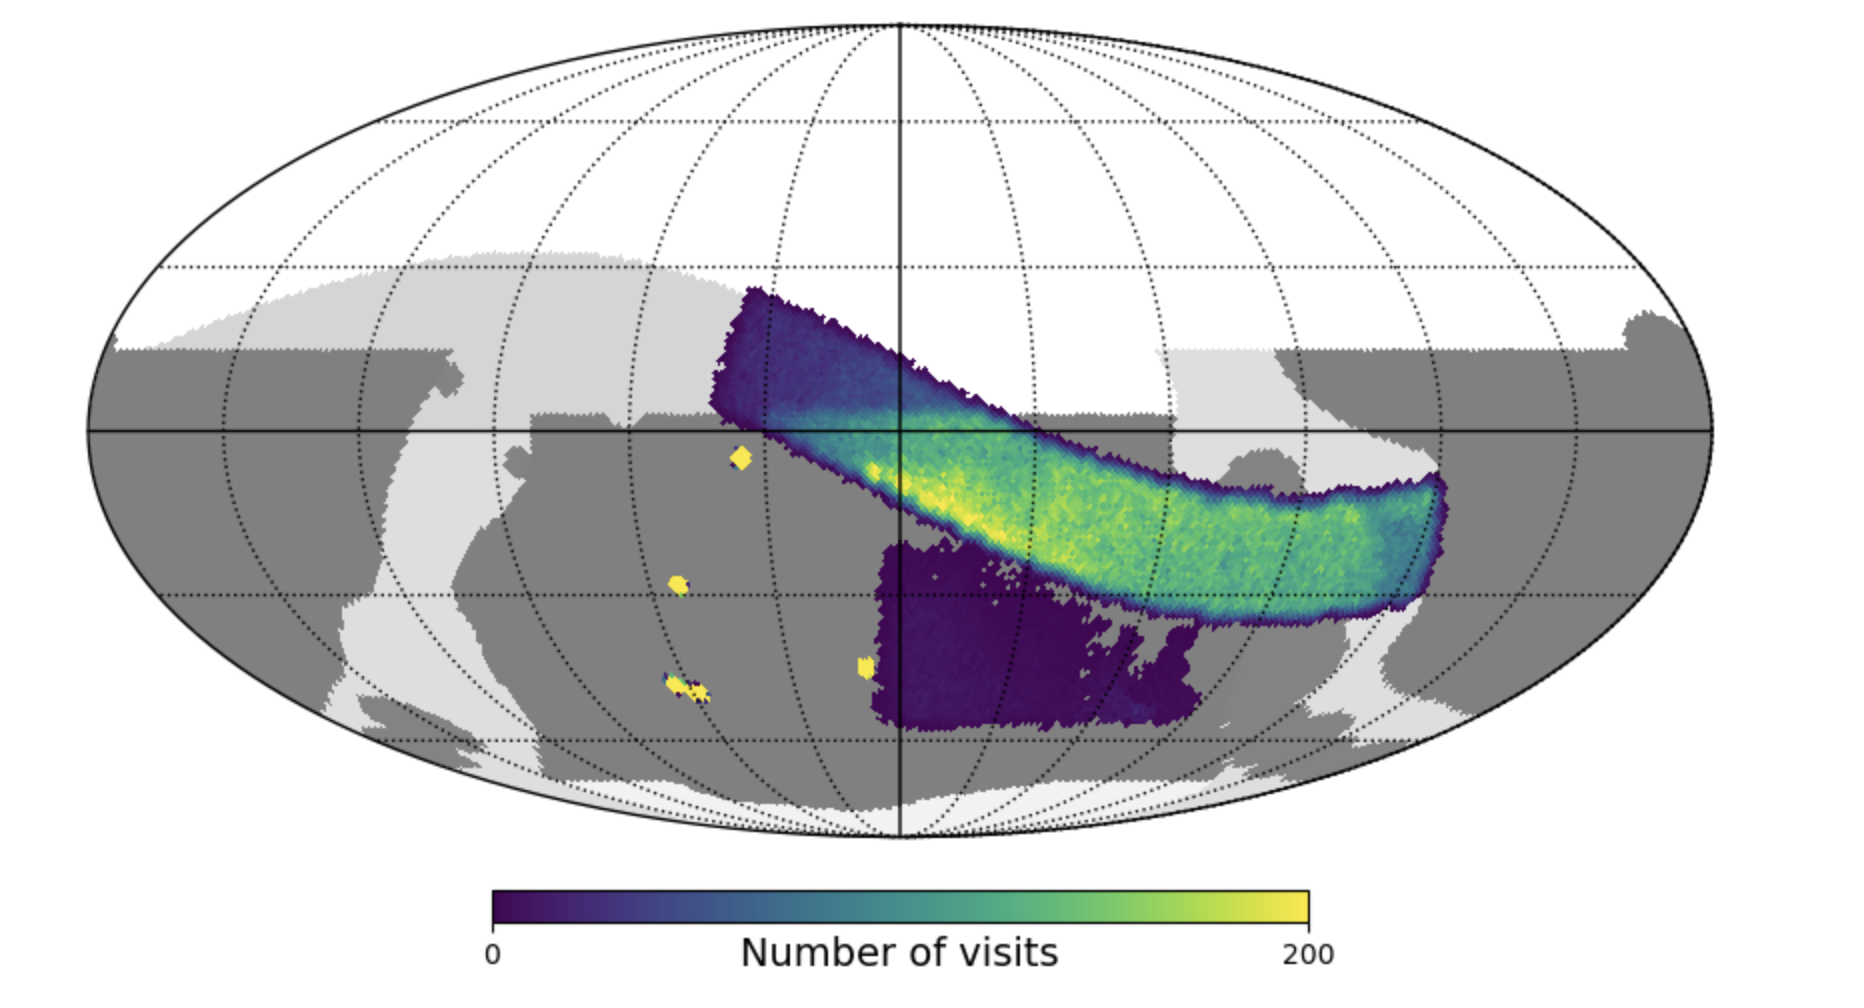
\includegraphics[width=1\textwidth]{./sv_surveys_coverage.png}
    \caption{SV surveys coverage expressed as total number of overlapping visits across the ugrizy bands.}
    \label{sv_surveys_coverage}
    \end{center}
\end{figure}

\begin{figure}[htbp]
    \begin{center}
    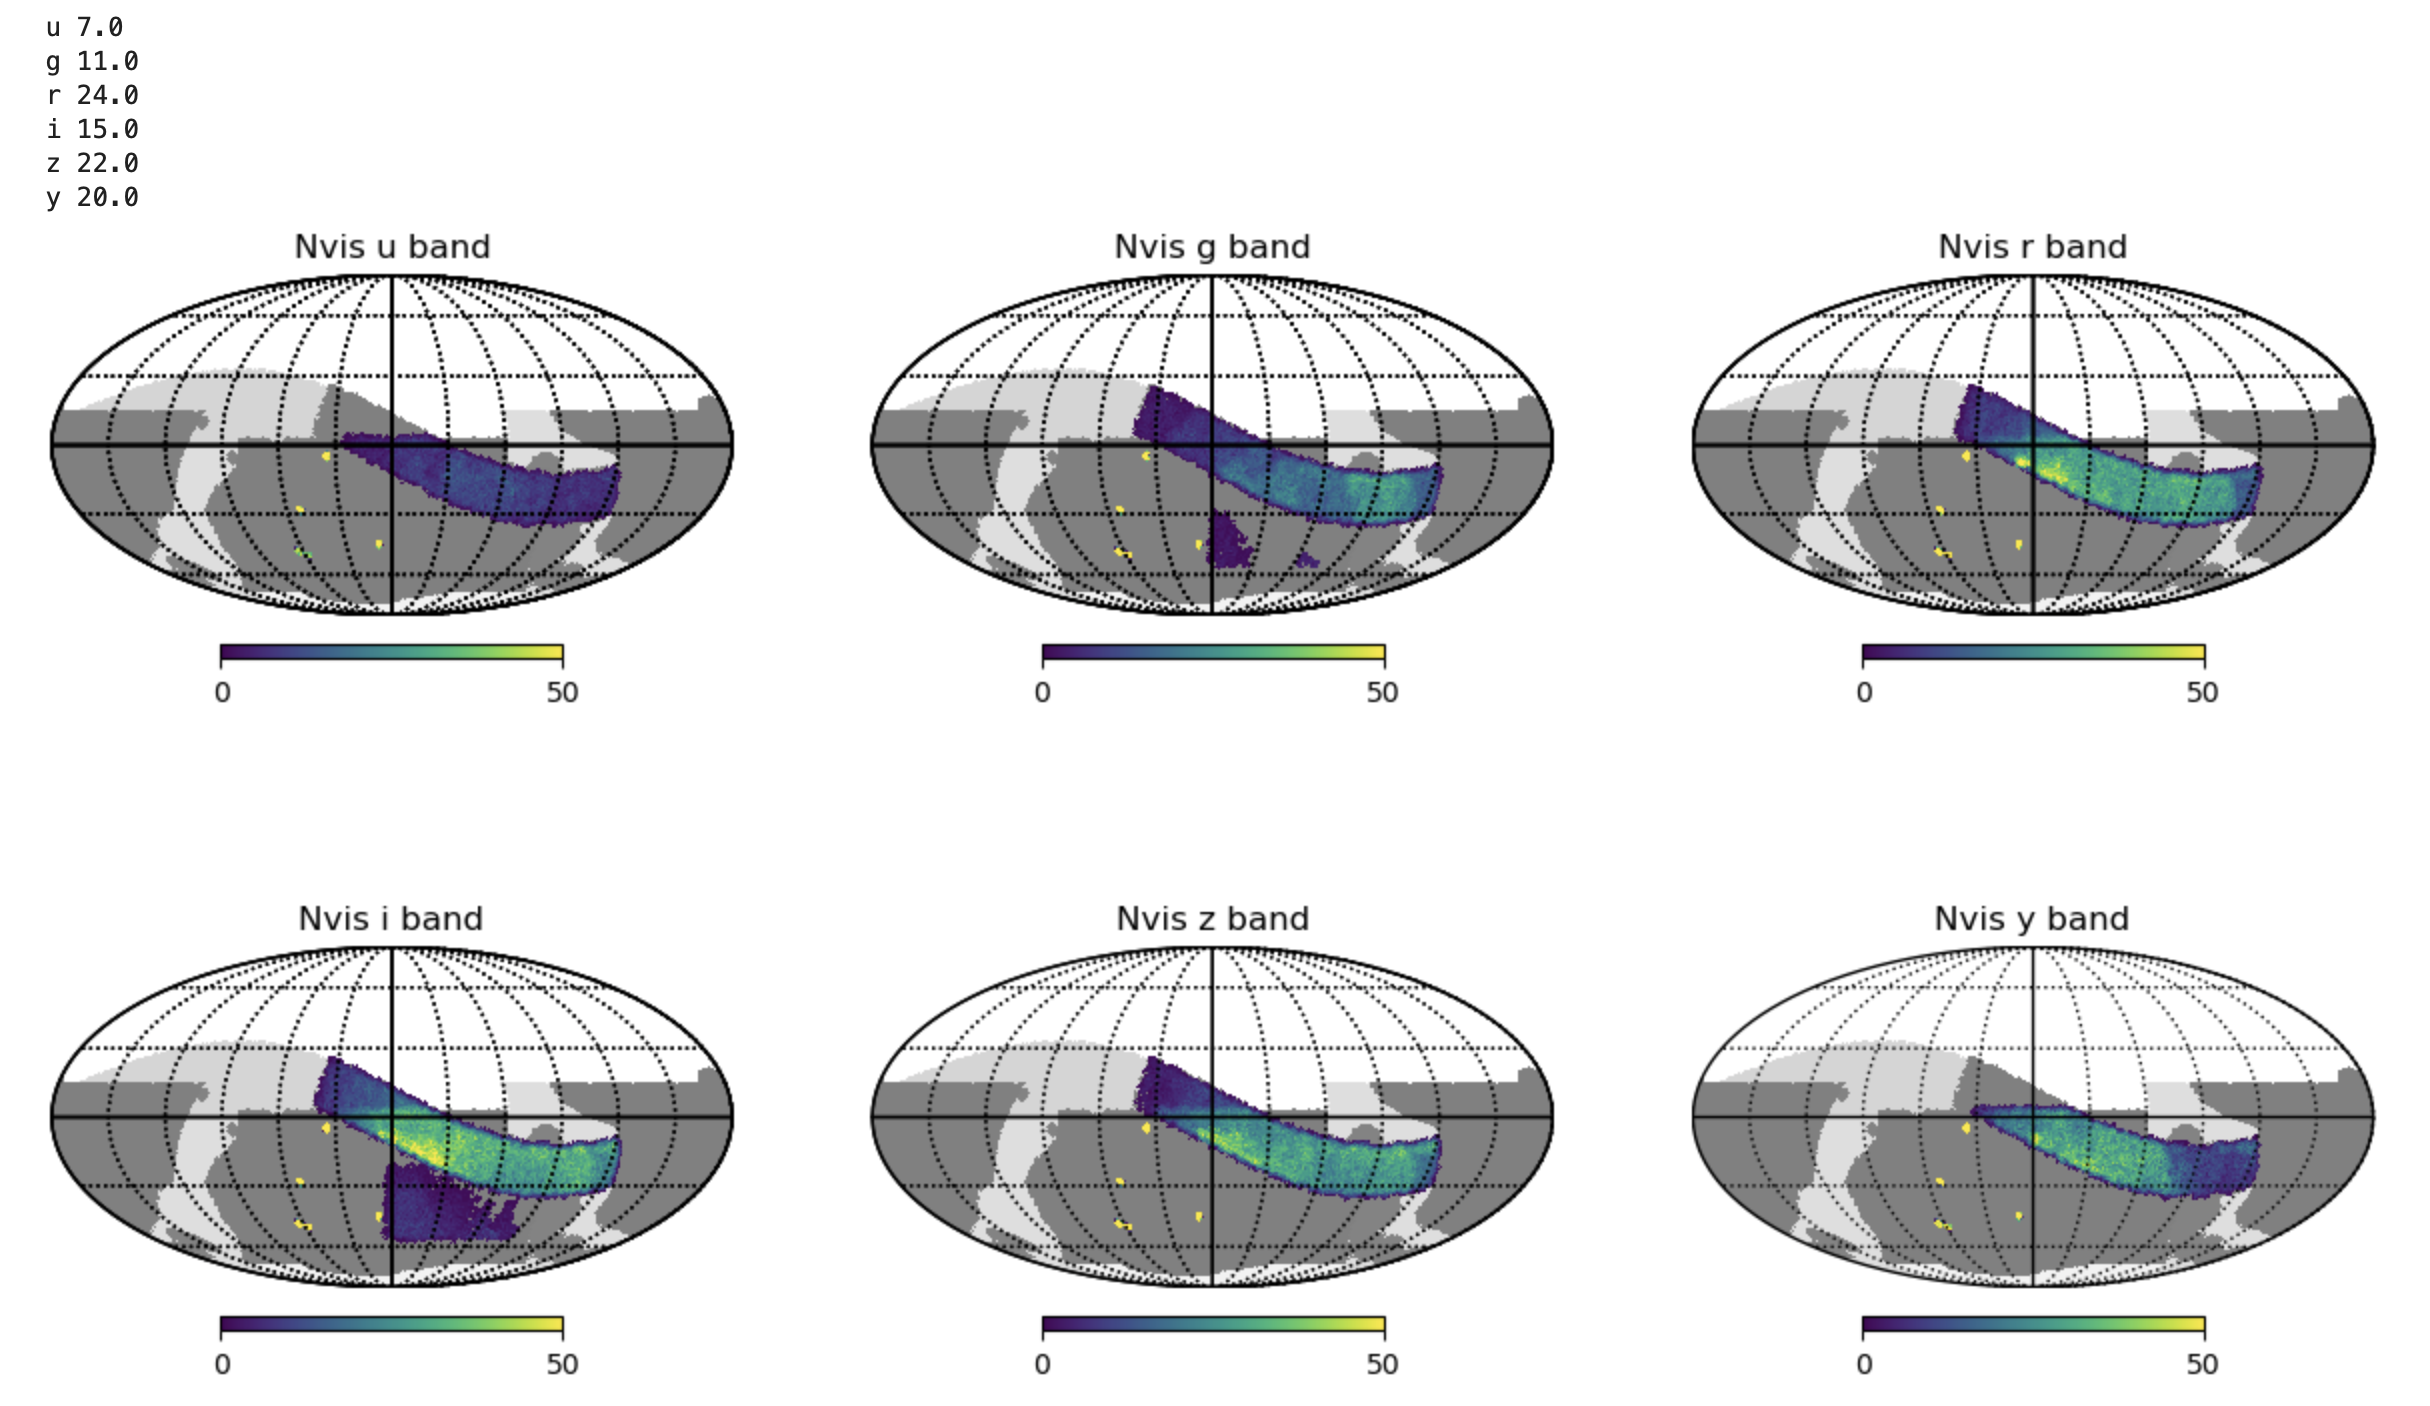
\includegraphics[width=1\textwidth]{./sv_surveys_coverage_band.png}
    \caption{SV surveys coverage expressed as total number of overlapping visits in each of the individual ugrizy bands.}
    \label{sv_surveys_coverage_band}
    \end{center}
\end{figure}

\begin{figure}[htbp]
    \begin{center}
    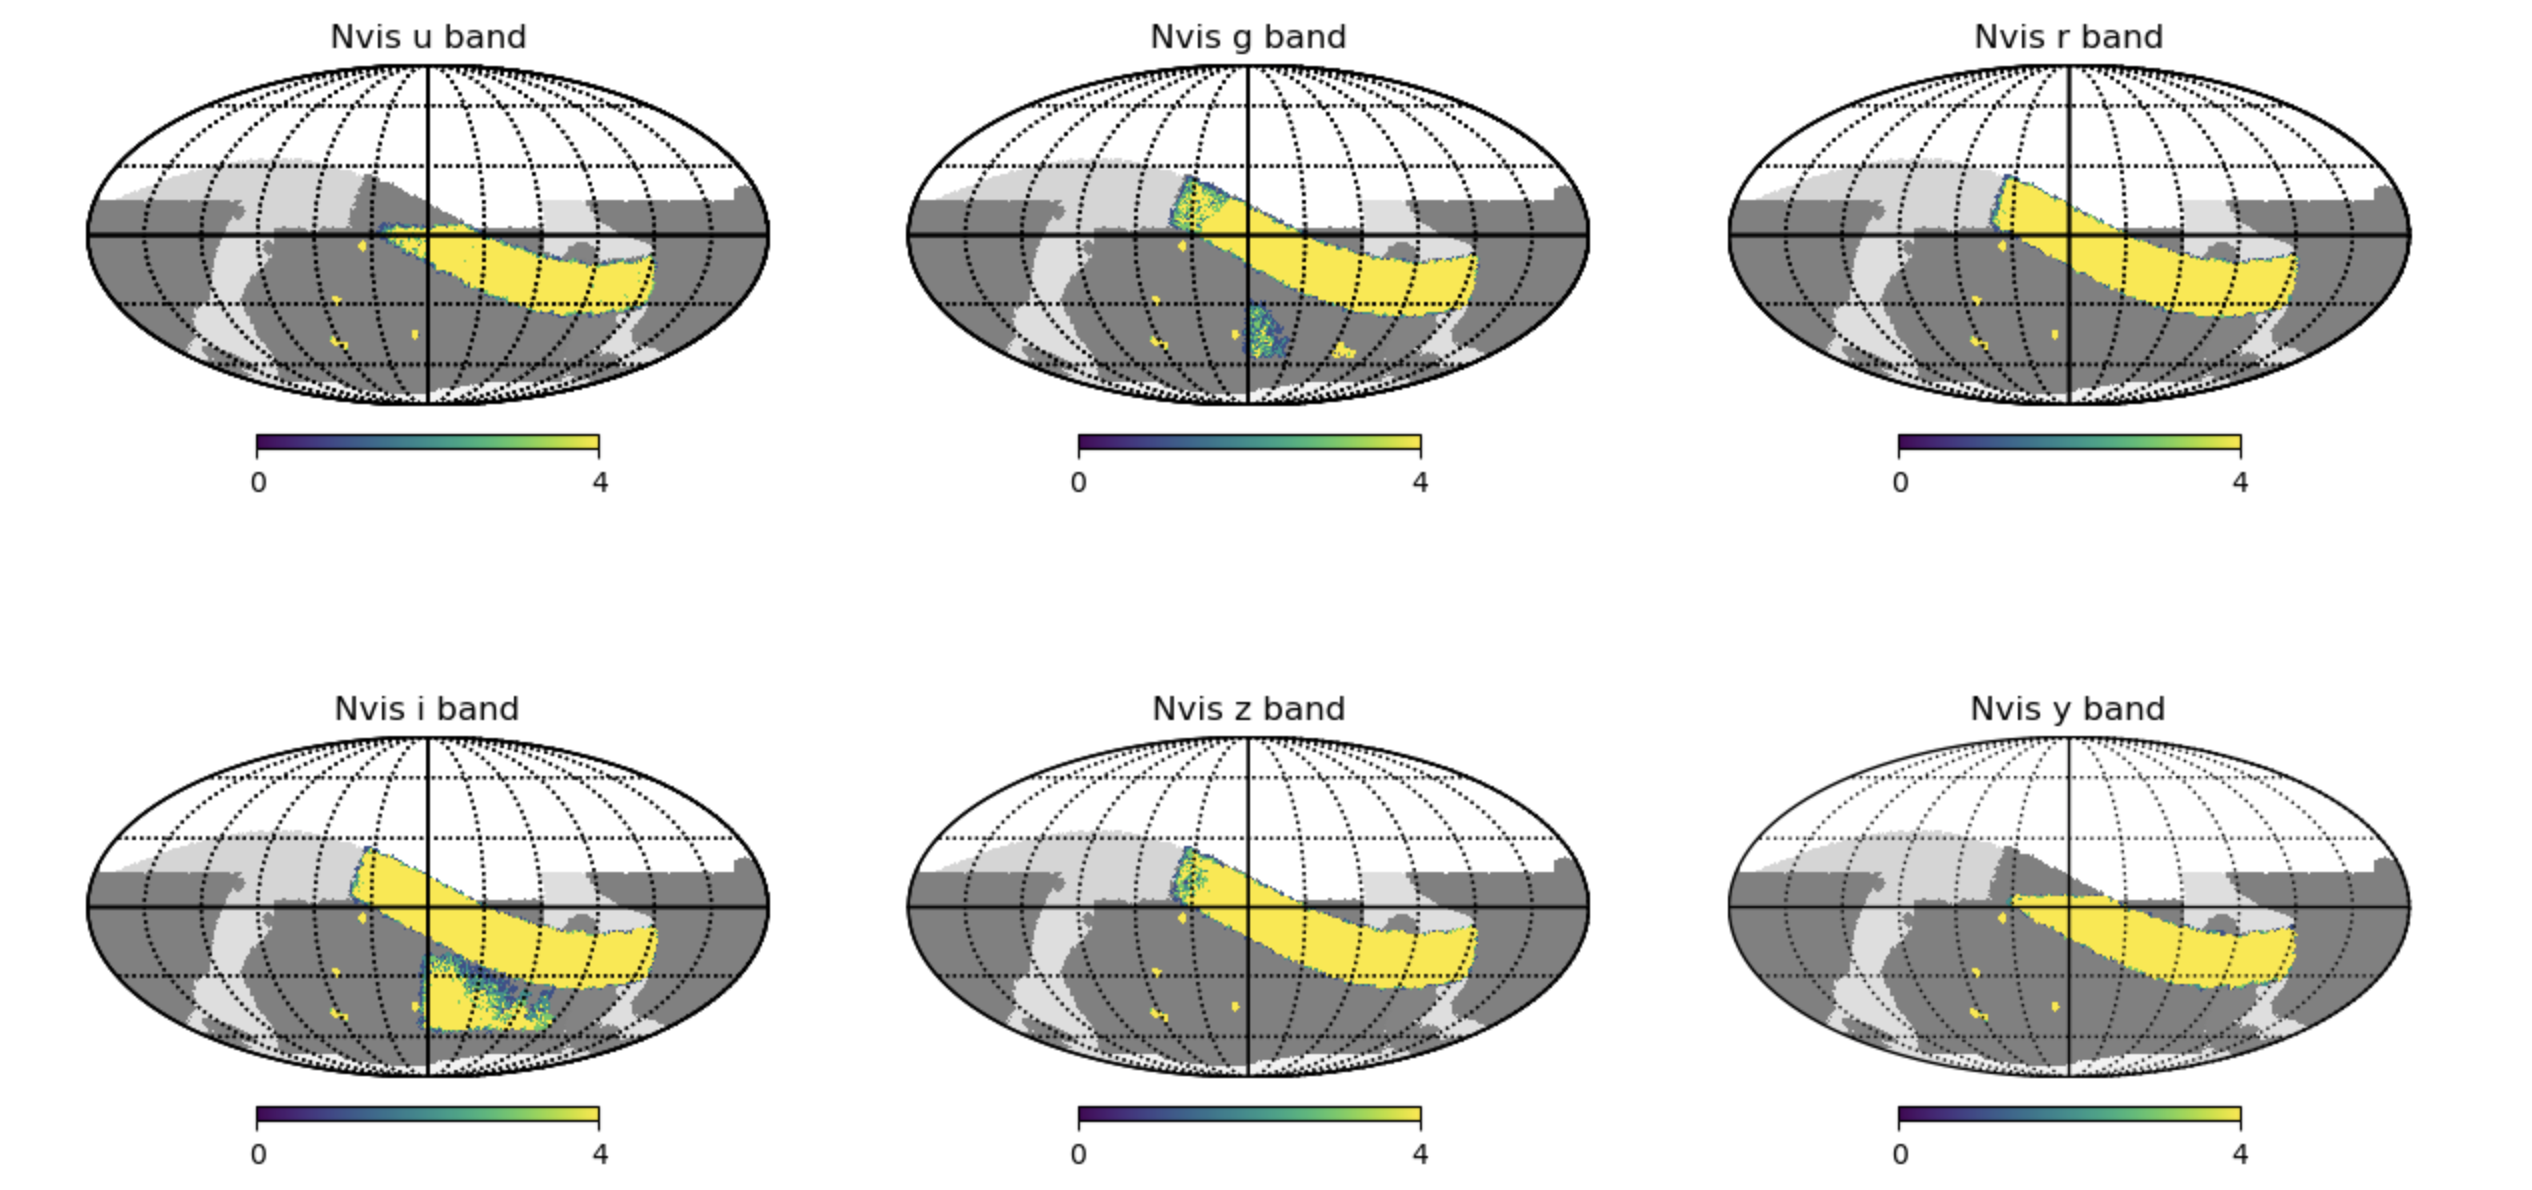
\includegraphics[width=1\textwidth]{./sv_surveys_template_coverage.png}
    \caption{SV surveys template coverage expressed as total number of overlapping visits in each of the individual ugrizy bands, with a color scale selected to more easily visualize template coverage.}
    \label{sv_surveys_template_coverage}
    \end{center}
\end{figure}

\begin{figure}[htbp]
    \begin{center}
    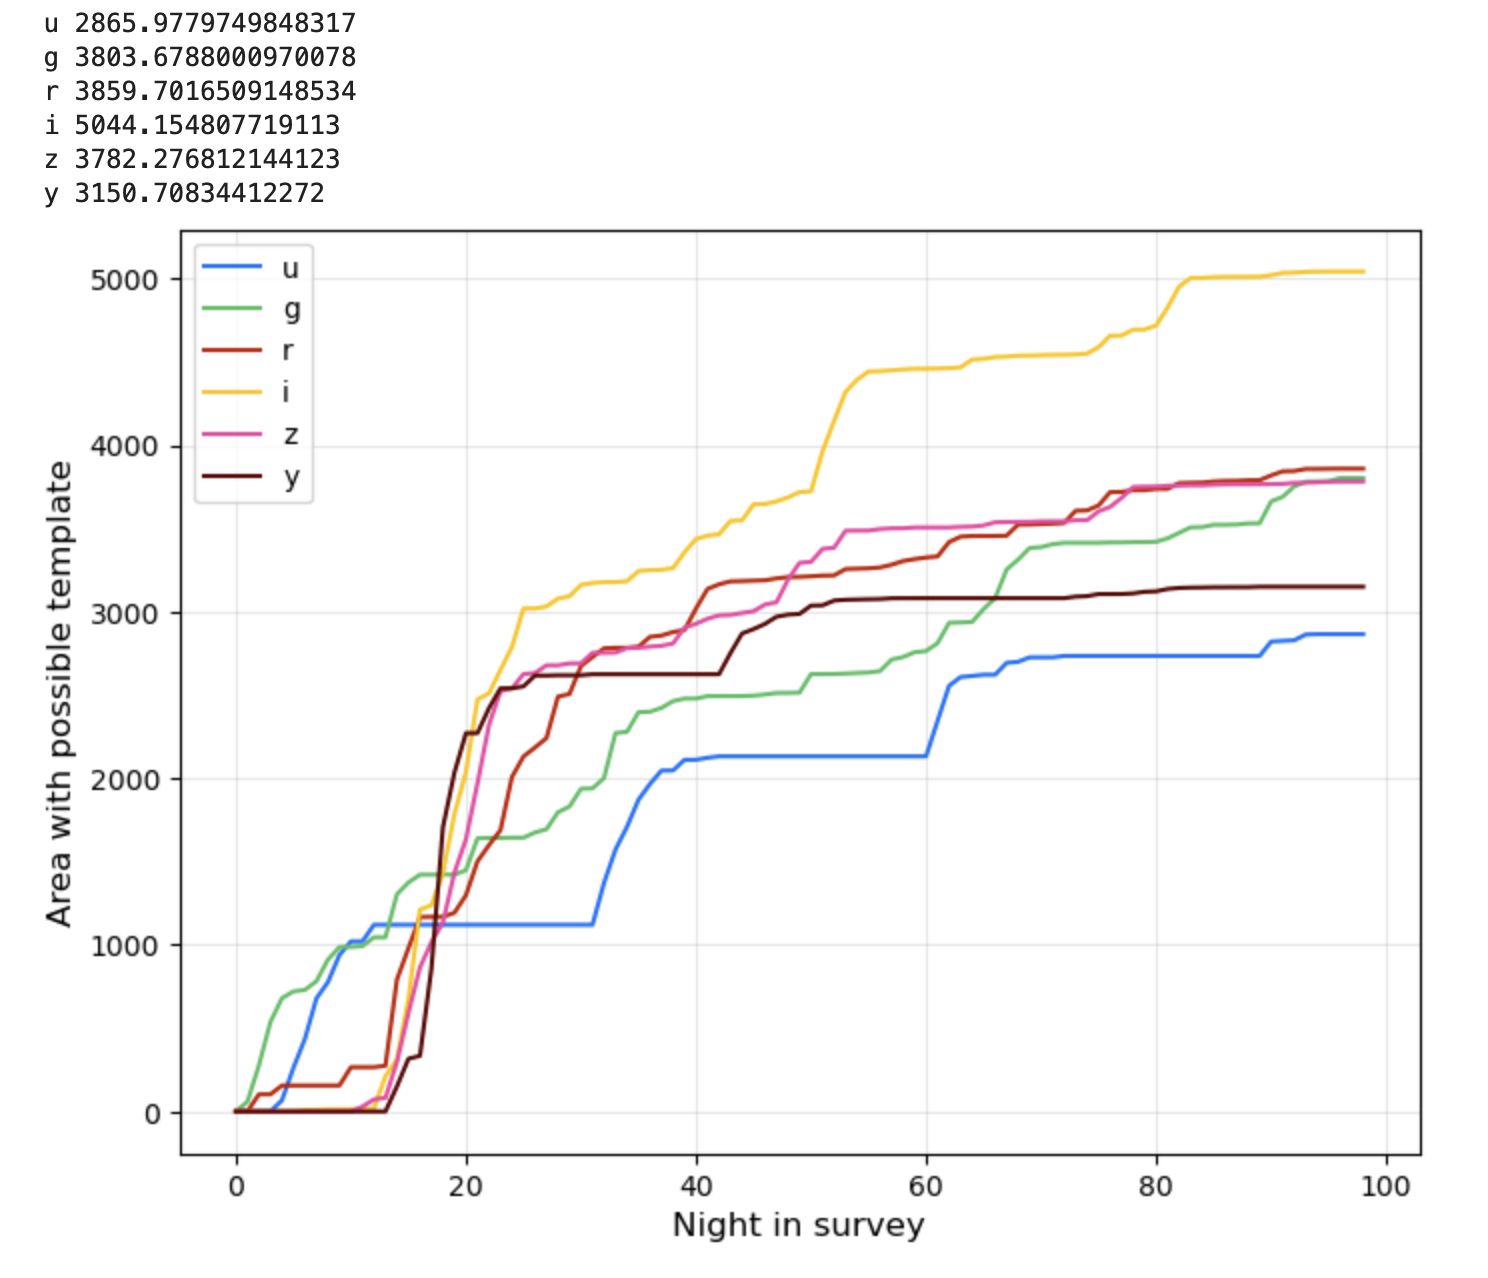
\includegraphics[width=1\textwidth]{./sv_surveys_cumulative_template_area.png}
    \caption{SV surveys coverage expressed as total number of overlapping visits in each of the individual ugrizy bands.}
    \label{sv_surveys_cumulative_template_area}
    \end{center}
\end{figure}

\textit{Deep Survey}

The Deep Survey is implemented using a configuration similar to that of the LSST DDFs, specifically, targeting the four DDFs located in the south Galactic cap that are visible in July-September: ELAIS S1, XMM LSS, ECDFS, and EDFSa + EDFSb.
The combined area of these four fields is $\sim50$~deg$^2$, noting that EDFS comprises two adjascent LSSTCam pointings.
Observations for the SV survey itself will be complemented by prior Rubin/LSSTCam observations of the COSMOS DDF in $ugrizy$ acquired in May-June 2025, for a combined coverage of $\sim60$~deg$^2$ considering all five LSST DDFs.
By design, the LSST DDFs overlap many existing and planned ground-based and space-based imaging and spectroscopic datasets, as well as broad multiwavelength datasets from radio to X-ray.
There is approximately $\sim30$~deg$^2$ of overlap with the Euclid Q1 release, and overlap with deep fields recommended by the Roman Observations Time Allocation Committee.
% https://arxiv.org/pdf/2505.10574

The planned observing cadence for the DDFs during the SV surveys uses a modified form of the ``ocean'' strategy currently being considered by the SCOC.
The ``ocean'' strategy features more frequent observing epochs to better sample night-to-night time-domain phenomena and provide more distinct epochs for validating the internal calibration during commissioning.
The primary modification for the SV surveys is to increase the number of visits relative to the baseline ``ocean'' strategy in order to accumulate a deeper integrated exposure during the finite time period of the SV surveys.
During the SV surveys, XMM LSS is designated for a ``deep season'', with longer sequences of visits in each epoch, particularly in the $i$ and $z$ bands.
ELAIS S1, ECDFS, and EDFS are designated for ``shallow seasons''.
Visits are split evenly across the EDFS A and B pointings.

\textit{Wide Survey}

The Wide Survey is implemented using a configuration similar to that of the LSST Wide-Fast-Deep, but constrained to a region of $\pm10$~deg in ecliptic latitude.
By concentrating the observations within this region, it is possible to build several hundred degrees of template coverage in multiple bands within the first month the SV survey, thus enabling survey-scale tests of Prompt Processing with difference image analysis during the SV surveys.
The ecliptic region is selected to test Solar System Object processing pipelines at LSST survey scale.
The planned footprint extends across the southern Galactic cap, touching the Galactic plane on one side, thus covering regions with a range of stellar densities and stellar populations, as well as a large contiguous low-dust region at high Galactic latitude.
The footprint spans a range of declinations, allowing access for other ground-based telescopes located in the southern and northern hemispheres.
The footprint coincides with the low-dust WFD, Galactic plane, and North Ecliptic Spur from the standard LSST Cadence, with a ratio of visits and band coverage in each region matching that of the standard LSST cadence.
For example, the band coverage in the low-dust WDF and Galactic plane is $ugrizy$, while the north ecliptic spur recieves a smaller total number of visits and limited to the $griz$ bands.

\begin{figure}[htbp]
    \begin{center}
    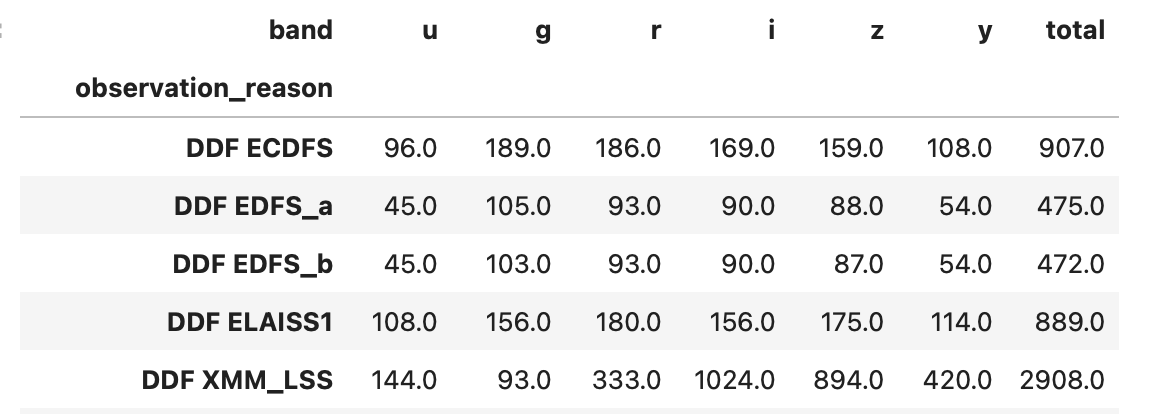
\includegraphics[width=1\textwidth]{./sv_surveys_ddf_visits.png}
    \caption{SV surveys total number of visits for the LSST DDFs in the south Galactic cap.}
    \label{sv_surveys_ddf_visits}
    \end{center}
\end{figure}

\begin{figure}[htbp]
    \begin{center}
    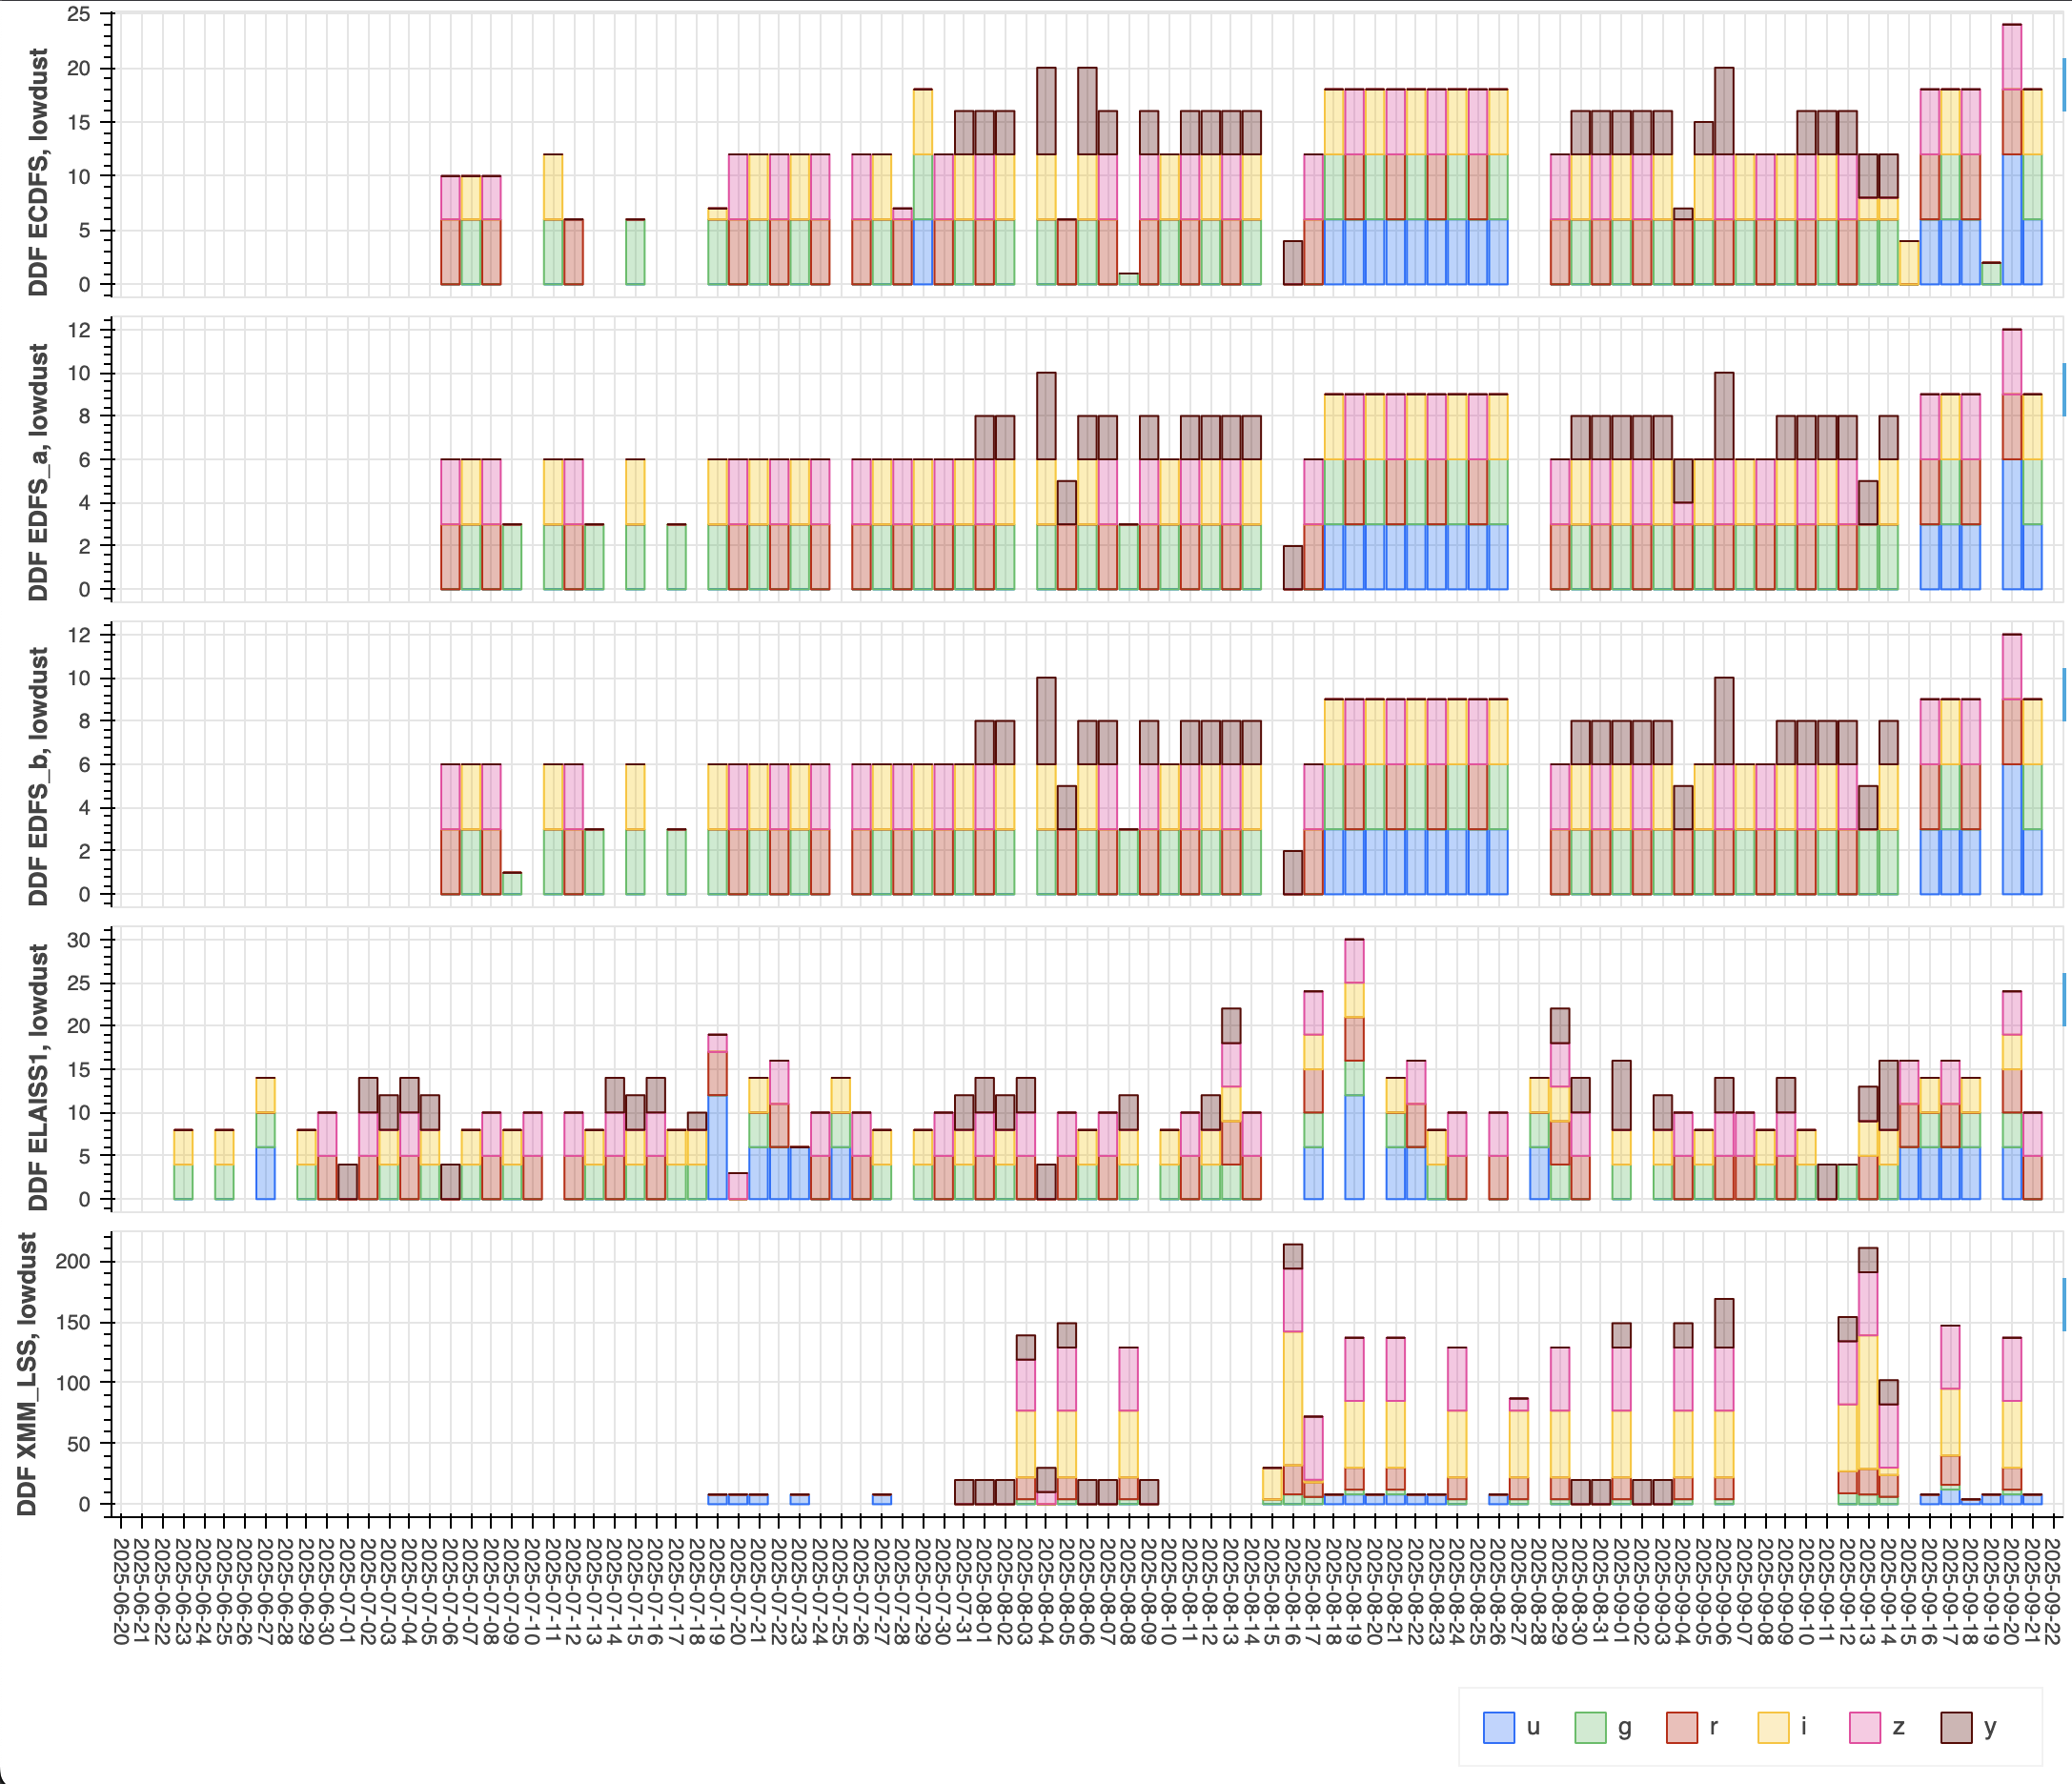
\includegraphics[width=1\textwidth]{./sv_surveys_ddf_cadence.png}
    \caption{SV surveys observing cadence for the LSST DDFs in the south Galactic cap.}
    \label{sv_surveys_ddf_cadence}
    \end{center}
\end{figure}


\textit{Expanded Template Generation Survey (Best Effort)}

In addition to the Deep Survey and Wide Survey, Rubin Observatory is exploring the technical feasibility of a \textbf{Expanded Template Generation Survey}, conducted on a best-effort basis, that would be optimized for expanding wide-area template coverage, including to support target-of-opportunity science cases during the first year of LSST.

The SV surveys are a Rubin Observatory Construction deliverable.
While the primary objective of the SV surveys is to fulfill the Construction Completeness criteria defined in this document, a secondary goal of the SV surveys is to facilitate a smooth transition to operations, and where possible, enhance the impact of the early Science Program.
Multiple science cases would benefit from acquiring wide-area template coverage during the on-sky commissioning period to enhance opportunities for time-domain science during the first year of LSST, including time-limited target-of-opportunity science cases that require contemporaneous observations with other facilities.
Accordingly, Rubin Observatory is exploring the technical feasibility of such observations as part of the SV surveys on a best-effort basis.

During system commissioning, telescope pointings at the end of night prior to dome closure are limited to an azimuth range in the southwest, thus limiting the capability to observe the LSST DDFs and the footprint of the Wide Survey.
During this end-of-night period, the current plans are to take observations to expand wide-area template coverage in 2 bands (likely $gi$) in regions located at declinations $[-55, -30]$ and Galactic latitudes $|b| > 15$~deg.
In the simulations presented here, the Expanded Template Generation Survey has been included in the same FBS configuration as the Wide and Deep Surveys, to assess the additional template coverage that could be achieved.

\begin{figure}[htbp]
    \begin{center}
    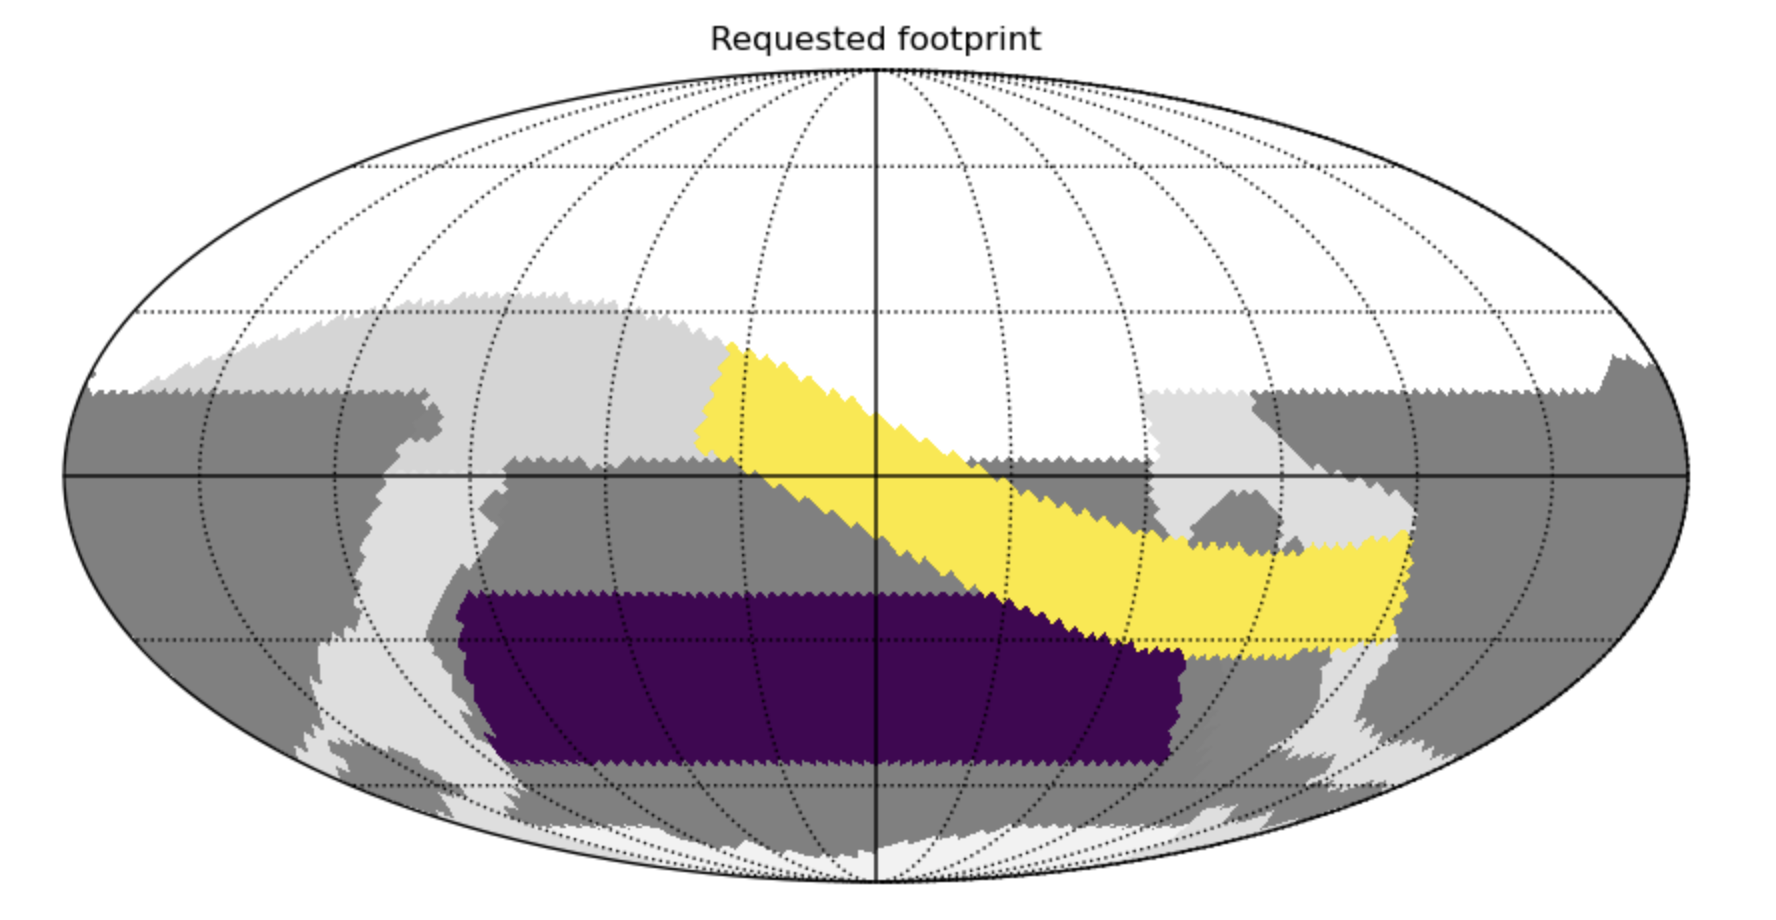
\includegraphics[width=1\textwidth]{./sv_surveys_requested_footprint.png}
    \caption{SV surveys requested footprint definition in equatorial coordinates. Yellow indicates the Wide Survey and purple indicates the Expanded Template Generation Survey. Gray shading indicates the standard LSST footprint.}
    \label{sv_surveys_requested_footprint}
    \end{center}
\end{figure}

\textit{Caveats}

The enhanced SV survey described here represents a design target based on system specifications.

Rubin Observatory is still in the commissioning phase; the key objective of the SV surveys is to directly verify the as-built system and to evaluate the operational efficiency under realistic conditions.
The actual volume of science-grade data collected will be directly related to the realized operational efficiency over the next several months, which includes uncertainty on the system-level performance, weather in Chilean winter, etc.
The actual volume of delivered science-grade data from the SV surveys might be a fraction of the design, and still be consistent with meeting the commissioning objectives.

If the realized operational efficiency during the pilot observations is lower than expected, the current plan is to reduce the footprint area by a corresponding amount to increase the likelihood that the integrated exposure design goals of the SV surveys can be achieved.

The defition of the SV Surveys is understood to be sufficiently broad to include all types of observations driven by the FBS that are suitable for performance evaluation of in-focus science images and Science Pipelines commissioning.

\subsection{Criteria for Completeness Description}

The Science Validation Surveys construction completeness criteria are considered to be met upon verification by analysis of the System Availability requirements described in the OSS.
The baseline is to conduct one or more scheduler-driven Science Validation surveys as the primary activity at the conclusion of the commissioning period, with the objective to verify system reliability over a minimum 30-day window coinciding with the Science Validation survey. This 30-day window is anticipated to begin around the System First Light milestone, although it could start somewhat before or after.
Verification of System Availability requirements includes

\begin{itemize}
        \item analysis of the operational uptime accounting for weather losses as well as scheduled and unscheduled system downtime and
        \item tests of the observing efficiency in terms of the rate of visits within scheduled observing time, including time intervals between visits for a nominal survey strategy (exposure time, slew time, readout time, filter exchange time) under the normal operating conditions defined in the OSS.
\end{itemize}

During the verification window, the commissioning team might choose to include some engineering activities to further optimize system performance. Planned engineering activities do not ``count against'' evaluation of the system reliability, so long as unplanned faults, etc., do not limit our ability to predictably operate the observatory.

A 30-day period of sustained on-sky observations, routinely delivering acceptable science-quality images, is considered the minimum to cover the range expected environmental conditions, provide sufficient opportunities for science verification, and demonstrate operational procedures.

Consistent Data Release Processing of the full dataset acquired during the Science Validation surveys, along with verification of the scientific performance at survey scale with the resultant data products, could continue in the period between the handover to Operations and CCR4 (Section \ref{sec:srd}), provided that the functionality to process and characterize on-sky observations has been demonstrated on smaller scales (Sections \ref{sec:dm} and \ref{sec:sdqa}).

The Operations team might decide to conduct more extended Science Validation Survey and/or further system optimization work during first months of operations - ``Scenario B'' described in Early Science Program \citeds{RTN-011}.

%The observatory should operate continuously in scheduler-driven mode for at least 10 days to demonstrate stable operation.
%The baseline plan with at least two months of Science Validation Surveys with would offer further opportunities for science validation and optimization of survey operations, likely enhancing the delivered data quality and observatory efficiency during Early Operations, as well as informing science pipeline development and refinements leading up to the production of LSST DR1.

\subsection{Pre-Operations Interactions}

In the current baseline schedule, the Science Validation surveys are the final activity prior to the acceptance of the Observatory by the Operations team.
The progress of the Science Validation surveys will be routinely monitored and communicated to the Operations team in the period leading up to the handover.
%Scheduler configurations and night plans for the on-sky observing campaigns will be made available to the Operations team.
%The Operations team has considered scenarios that would continue the Science Validation surveys, or otherwise augment observing campaigns from the on-sky commissioning,
%in order to further test operational procedures and

The Science Validation Surveys represent an important opportunity to transfer knowledge of operational procedures to the Operations team.
In practice, a substantial fraction of Operations team personnel hold similar roles in the Construction project.
It is therefore anticipated that many Operations team members will be directly involved in running the Science Validation Surveys.
%, and rehearsing all major aspects of the 24-hour operations cycle in close coordination with the commissioning effort.

%At the conclusion of the Science Validation Survey(s), roughly two years will have elapsed since the start of Early System Integration and Testing, which places the LSST Observatory on schedule for its 2-year major maintenance and servicing.

%M1M3 Mirror Recoating: Remove, strip, clean, and re-coat the M1M3 mirror surfaces. Reinstall M1M3 mirror back into telescope. Associated activities include:

%\begin{itemize}
%\item Remove Top-End Integrating Structure with Camera and transfer to Summit Facility camera lab.
%\item Install camera dummy mass to allow the telescope to point to zenith for removal of the M1M3 mirror cell. Remove M1M3 mirror assembly and transfer to Summit Facility re-coating plant.
%\item Strip old coating, clean and re-coat mirror surfaces.
%\item Re-install M1M3 in telescope and prepare to receive the top-end integrating structure with the camera.
%\end{itemize}

%Camera Maintenance and Servicing: Clean, service, perform maintenance, and replace shutter. Associated activities include:

%\begin{itemize}
%\item Replace camera shutter with fresh operational unit;
%\item Inspect, service, or repair filter mechanisms;
%\item Clean internal camera optics;
%\item Inspect, service, and repair utility trunk electronics
%\end{itemize}

\subsection{Artifacts for Completion}

\begin{itemize}
\item Safety report from continuous observatory operations during the survey(s)
\item Summary of daytime and nighttime activity for each 24 hour period of the survey(s)
\item Metrics for the effective survey speed, including number of visits per night, telescope slew angles and slew times, filter changes, etc., which can be used to inform survey strategy during early operations
\item Characterization of the distribution of data quality delivered by the as-built system, for example, distributions of single-visit image quality and image depth
\item Realtime alert stream
\item Associated Data Release Production products accessed via the Rubin Science Platform (RSP)
\item Observatory maintenance report summarizing the pre-operations engineering activities and status of the observatory
\item Documentation for observatory operations, including recommendations for optimization of data quality and survey efficiency
\item Documentation for Data Facility operations
\end{itemize}
